\scanpage{68}
\deleted{\unsure{Cela posé}} Cette relation est évidemment \deleted{\unsure{symétrique}}\inserted{réflexive}, et
elle est transitive grâce au fait que
\[
\pi_0(\Sigma_{(2)})\longrightarrow
(\pi_0(\Sigma_{(1)}),\pi_0(\uline{b}))\times_{\pi_0(\Sigma_{(0)})}
(\pi_0(\Sigma_{(1)}),\pi_0(\uline{s}))
\]
est surjective, ce qui est facile à prouver,
grâce à l'hypothèse que $\uline{b}$ est fibrant, par le
\uline{Lemme} : Soit
\diagram{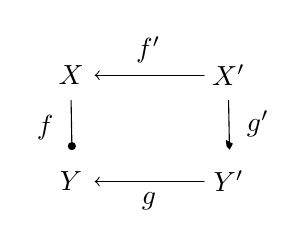
\begin{tikzpicture}[x=1cm,y=1cm,line cap=round,line join=round]
\node at (0,1.35) {$X$};
\node at (2,1.35) {$X'$};
\node at (0,0) {$Y$};
\node at (2,0) {$Y'$};
\draw[<-] (0.30,1.35)--(1.69,1.35);
\node[above] at (0.98,1.38) {$f'$};
\draw[<-] (0.30,0)--(1.69,0);
\node[below] at (0.99,-0.02) {$g$};
\draw (0,1.03)--(0.01,0.47);
\fill (0.01,0.45) circle (0.052);
\node[left] at (-0.10,0.69) {$f$};
\draw (2,1.03)--(2.01,0.50);
\fill (1.965,0.53)--(2.055,0.48)--(2.015,0.405)--(1.975,0.445)--cycle;
\node[right] at (2.11,0.73) {$g'$};
\end{tikzpicture}}
un carré
cartésien d'espaces top, avec $f$ fibrant,
alors $\pi_0(X')\longrightarrow\pi_0(X)\times_{\pi_0(Y)}\pi_0(Y')$ est surjectif
Ceci posé, considérons la catégorie top. discrète \unsure{associé|associée}
à l'ens \inserted{pré}ordonné \unsure{$I$\inserted{$=\pi_0(\Sigma_0)$},|$I_0$\inserted{$=\pi_0(\Sigma_0)$}} que par abus de langage
\inserted{[\unsure{anglicisme}\unsure{)|]}}
on \unsure{désignera|désigne} par $I$. On a alors un foncteur
\inserted{canonique} de catégories topologiques \deleted{\unsure{canoniques|canonique}}
\[
\uline{\Sigma}\xrightarrow{\uline{\varphi}}I
\]
qui est donc donné par des applications continues
\[
\left\{\begin{aligned}
\Sigma_{(0)}&\xrightarrow{\varphi_0}I_0=I\\
\Sigma_{(1)}&\xrightarrow{\varphi_1}I_1=\text{graphe de la relation d'ordre}
\end{aligned}\right.
\]
\inserted{$=\text{image de }\pi_0(\Sigma_1)$
\deleted{dans $\unsure{\pi_0(\Sigma_1)\times I|\pi_0(\Sigma_0)\times\Sigma_1}$}
dans $\pi_0(\Sigma_0)\times\pi_0(\Sigma_0)=I$}
i.e. des décompositions en sommes directes
\[
\Sigma_{(0)}=\coprod_{i\in I}\Sigma_i
\]
\[
\Sigma_{(1)}=\deleted{\unsure{\Sigma}}\coprod_{\substack{i,\unsure{j|g}\in I\\i\leq j}}\Sigma_{ij}
\]
\margin{\uline{NB} on suppose \uline{les} comp. connexes des $\Sigma_0$ et $\Sigma_1$ ouvertes}
compatibles avec $\uline{s}\ \uline{b}$
i.e $\uline{s}:\Sigma_{ij}\mathrel{-}\Sigma_i$
$\uline{b}:\Sigma_{ij}\mathrel{-}\Sigma_j$
avec $\Sigma_{(0)}\xrightarrow{\delta}\Sigma_{(1)}$ ($\delta(x)=\deleted{\unsure{\operatorname{id}^{\uline{\Sigma}}_x}}\operatorname{id}^{\uline{\Sigma}}_x$)
appliquant $\Sigma_i$ dans $\Sigma_{ii}$, \deleted{\unsure{et ainsi}} (ce qui
implique déjà la compatibilité de $\uline{\varphi}=(\varphi_0,\varphi_1)$ avec
la composition). De plus, $\uline{\varphi}$ est un
\margin{67}
